\documentclass{beamer}
\usepackage[utf8]{inputenc}
\usepackage[T1]{fontenc}
\usepackage{lipsum, lmodern}
\usepackage[scaled=.95]{helvet}% helvetica as the origin of arial
\usepackage[helvet]{sfmath}    % for the mathematical enviroments
\usepackage{xcolor} % For color
\renewcommand{\familydefault}{\sfdefault}

%% ETH beamer theme
% Options: [default]
%   itemsblack/[itemsblue]: change color of bullets etc. to black/blue in itemize style environments
%   [titlesblack]/titlesblue: change color of frame titles/subtitles to black/blue
% \usetheme[itemsblack,titlesblack]{eth}
\usetheme{eth}

%% Theme uses ETH blue color by default. Can be changed to any color using this command: 
% \setbeamercolor{structure}{fg=blue}

%% Mandatory variables
\author{Jonathan Burkhard}
\title{Design and Control of a Bicopter MAV}
\date{\today}

%% Optional variables
% \Presentationsupervisor{Jane Smith} % for one supervisor
\supervisors{Dr. Zachary Taylor, Karen Bodie and Prof. Dr. R. Siegwart} % for multiple supervisors
% \projecttype{Master's Thesis}

\begin{document}
\frame{\maketitle}
\begin{frame}{Table of contents}{Subtitle}
	\tableofcontents
\end{frame}

\section{Literature}
\begin{frame}{From the litterature}
\begin{itemize}
\item Read some litterature 
\item Read some websites on "Do it yourself"
\item Read some slides from lecture of Robots dynamics
\end{itemize}
\begin{figure}
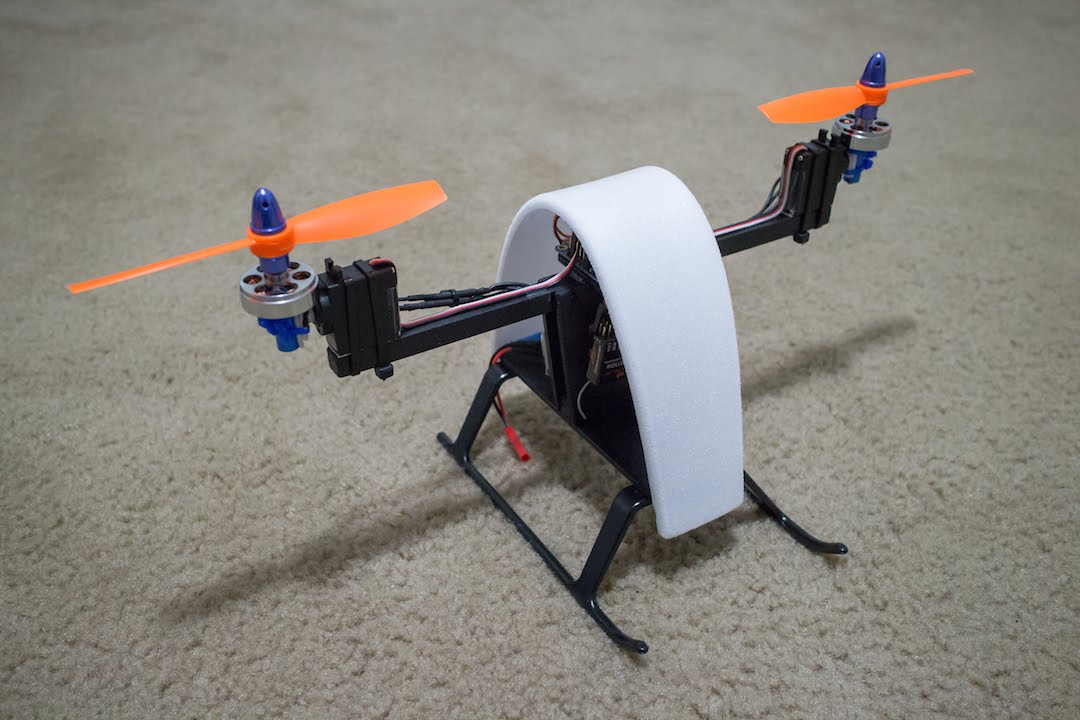
\includegraphics[scale=0.1]{pictures/bicopter}
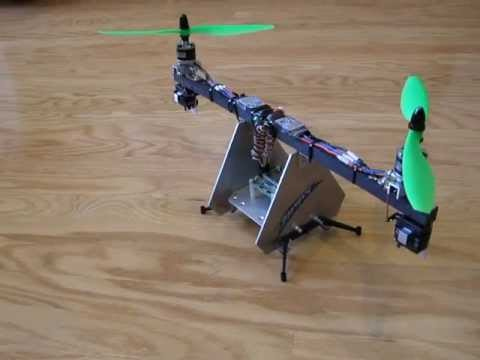
\includegraphics[scale=0.2]{pictures/bicopter2}
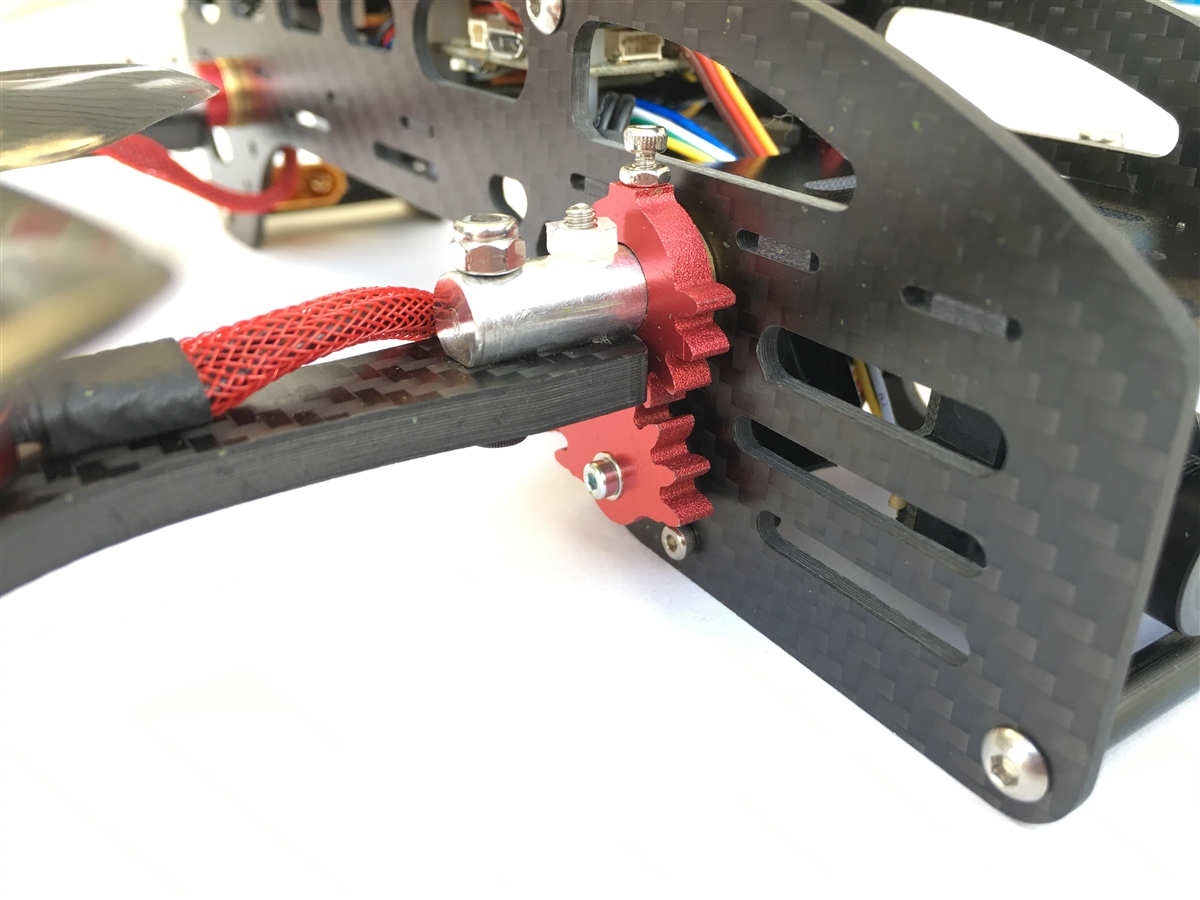
\includegraphics[scale=0.11]{pictures/bicopter3}
\caption{Different existing parts}
\end{figure}
\end{frame}

\section{Design of the Bicopter}
\begin{frame}{Design of the Bicopter}
The goal of the design is to
\begin{itemize}
\item be simple
\item use the maximum of commercially avaible parts
\end{itemize}
\begin{figure}
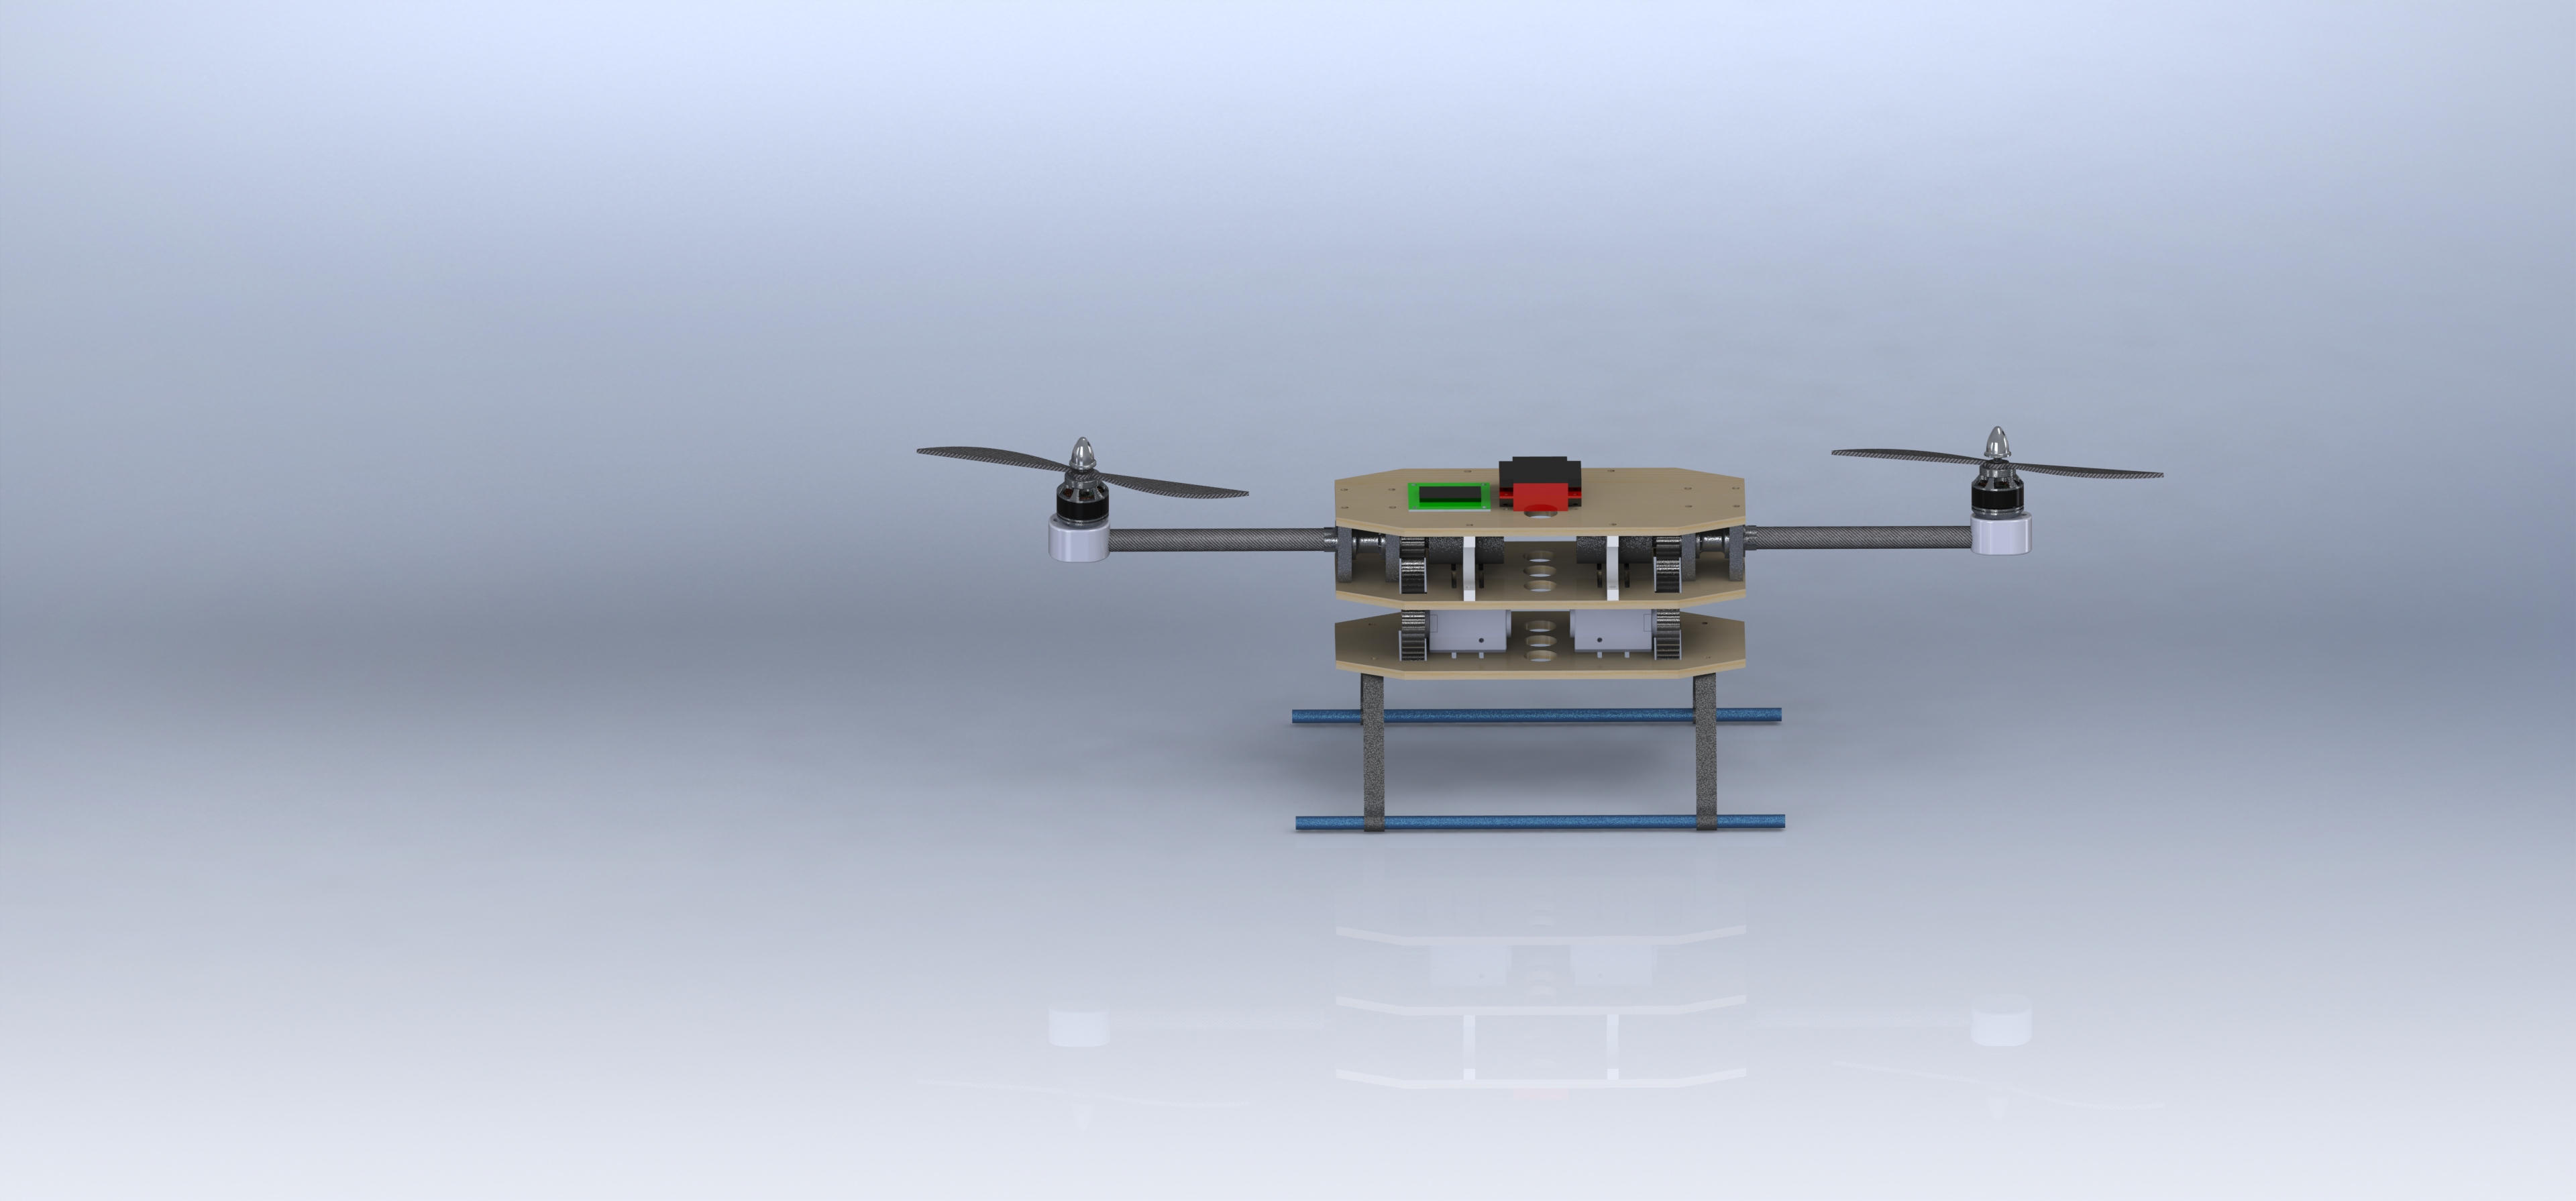
\includegraphics[scale=0.07]{pictures/picture4}
\end{figure}
\end{frame}

\begin{frame}{Design of the Bicopter}
A few numbers:
\begin{itemize}
\item Tilting motor has 60 RPM and is increased with gearings to 120 RPM
\item Slip-ring with 3 wires
\item Battery life of over 5 minutes
\end{itemize}
\begin{figure}
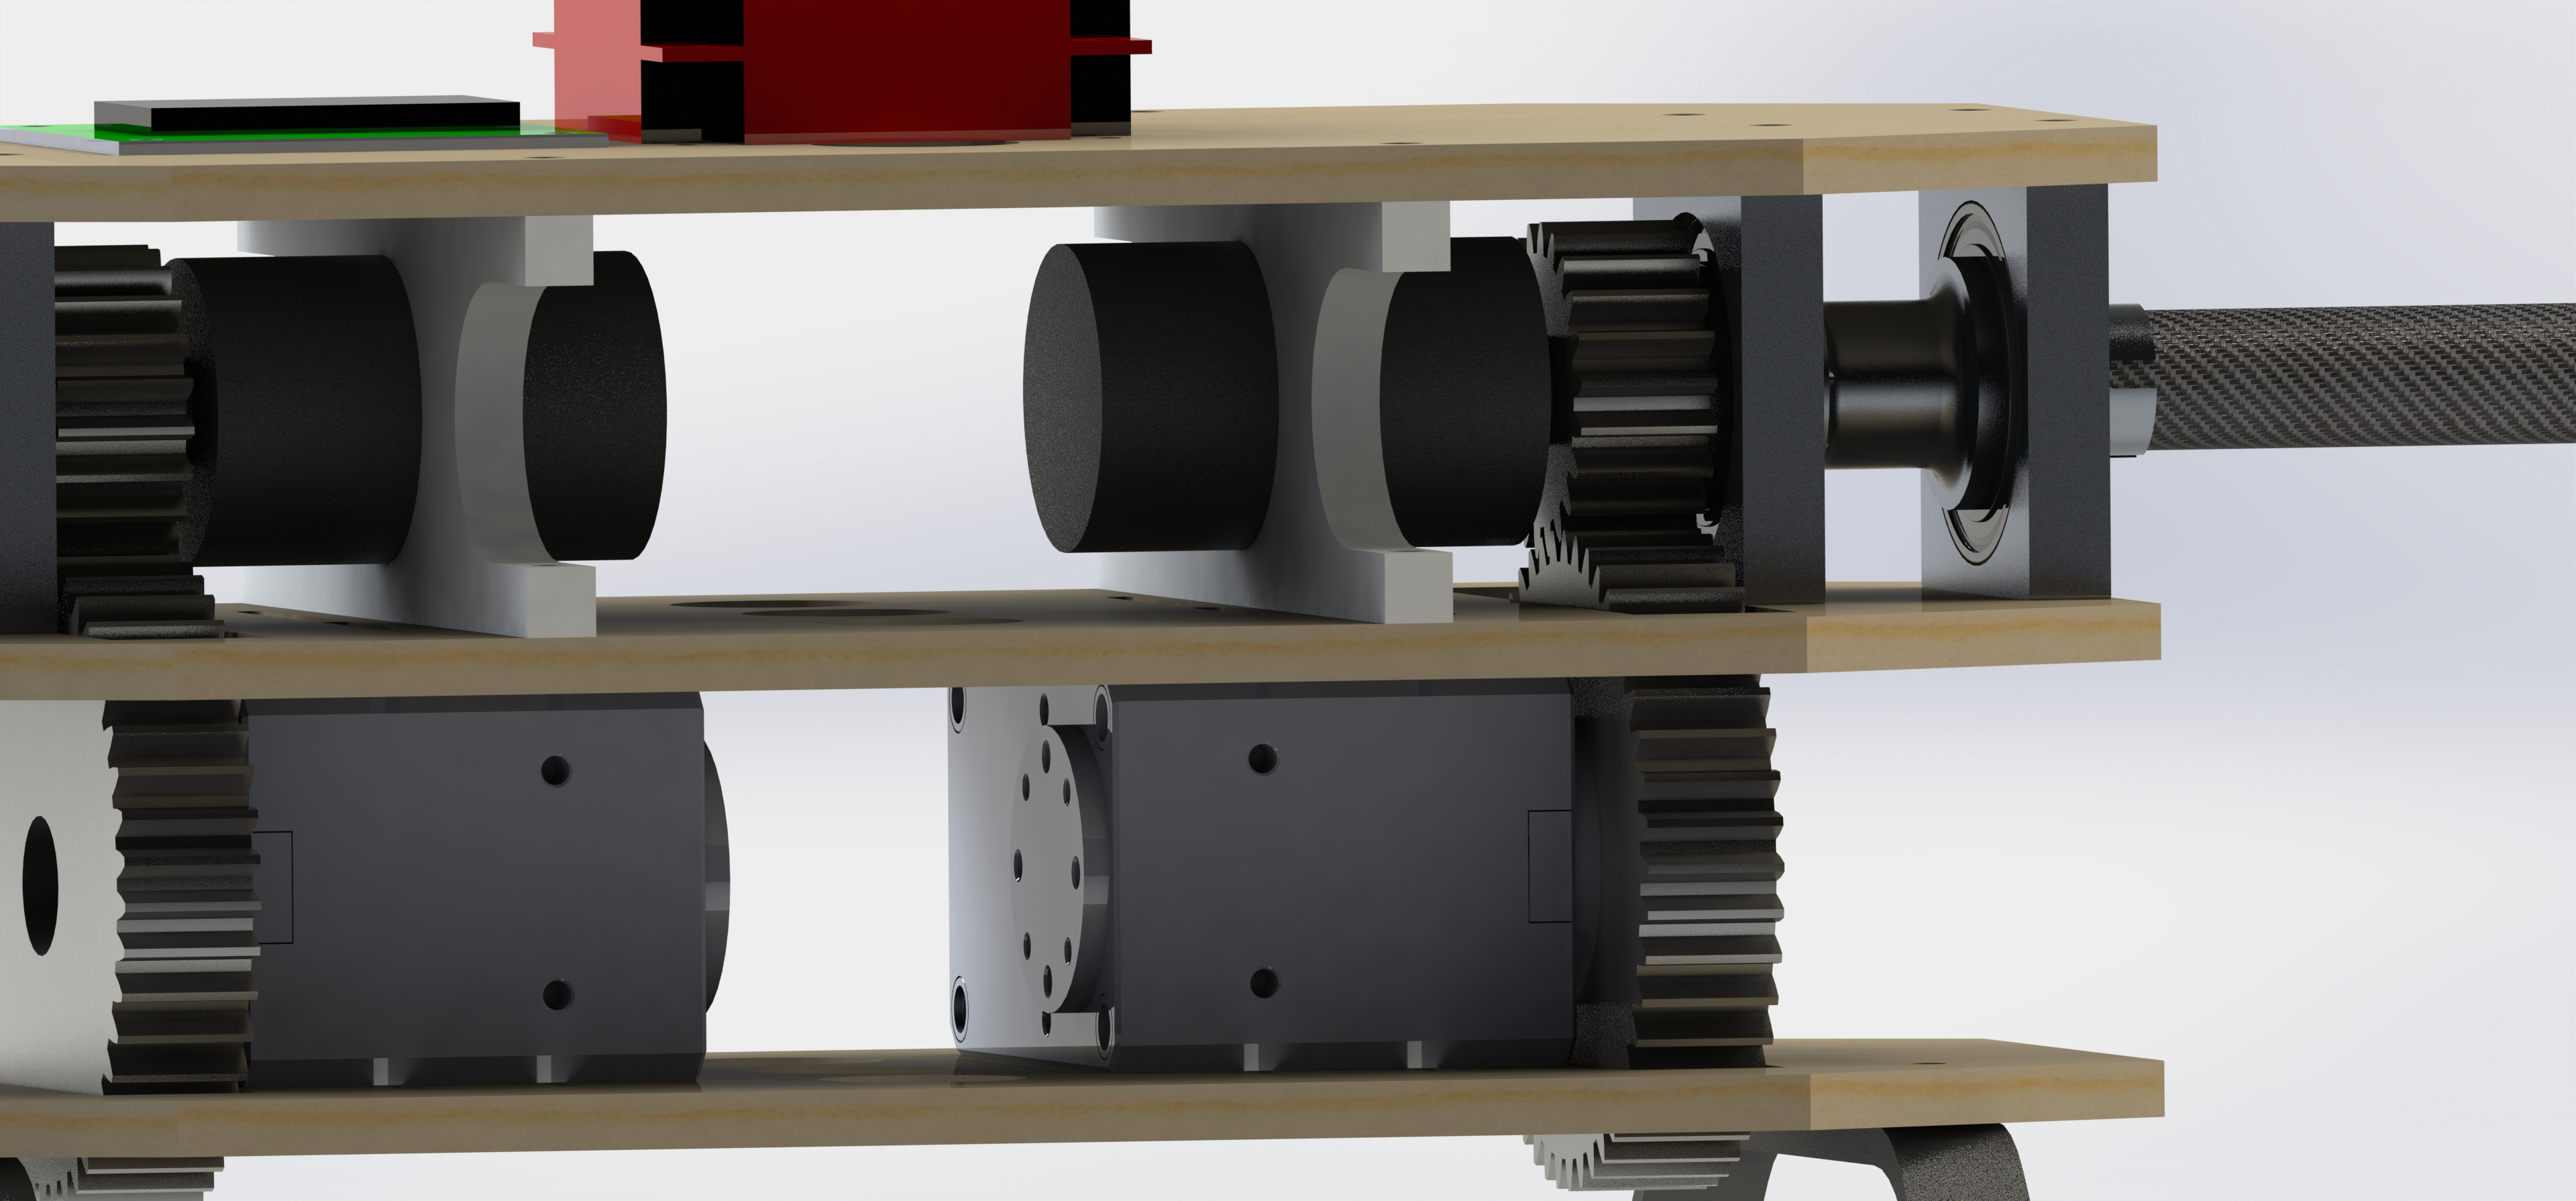
\includegraphics[scale=0.04]{pictures/zoom1}
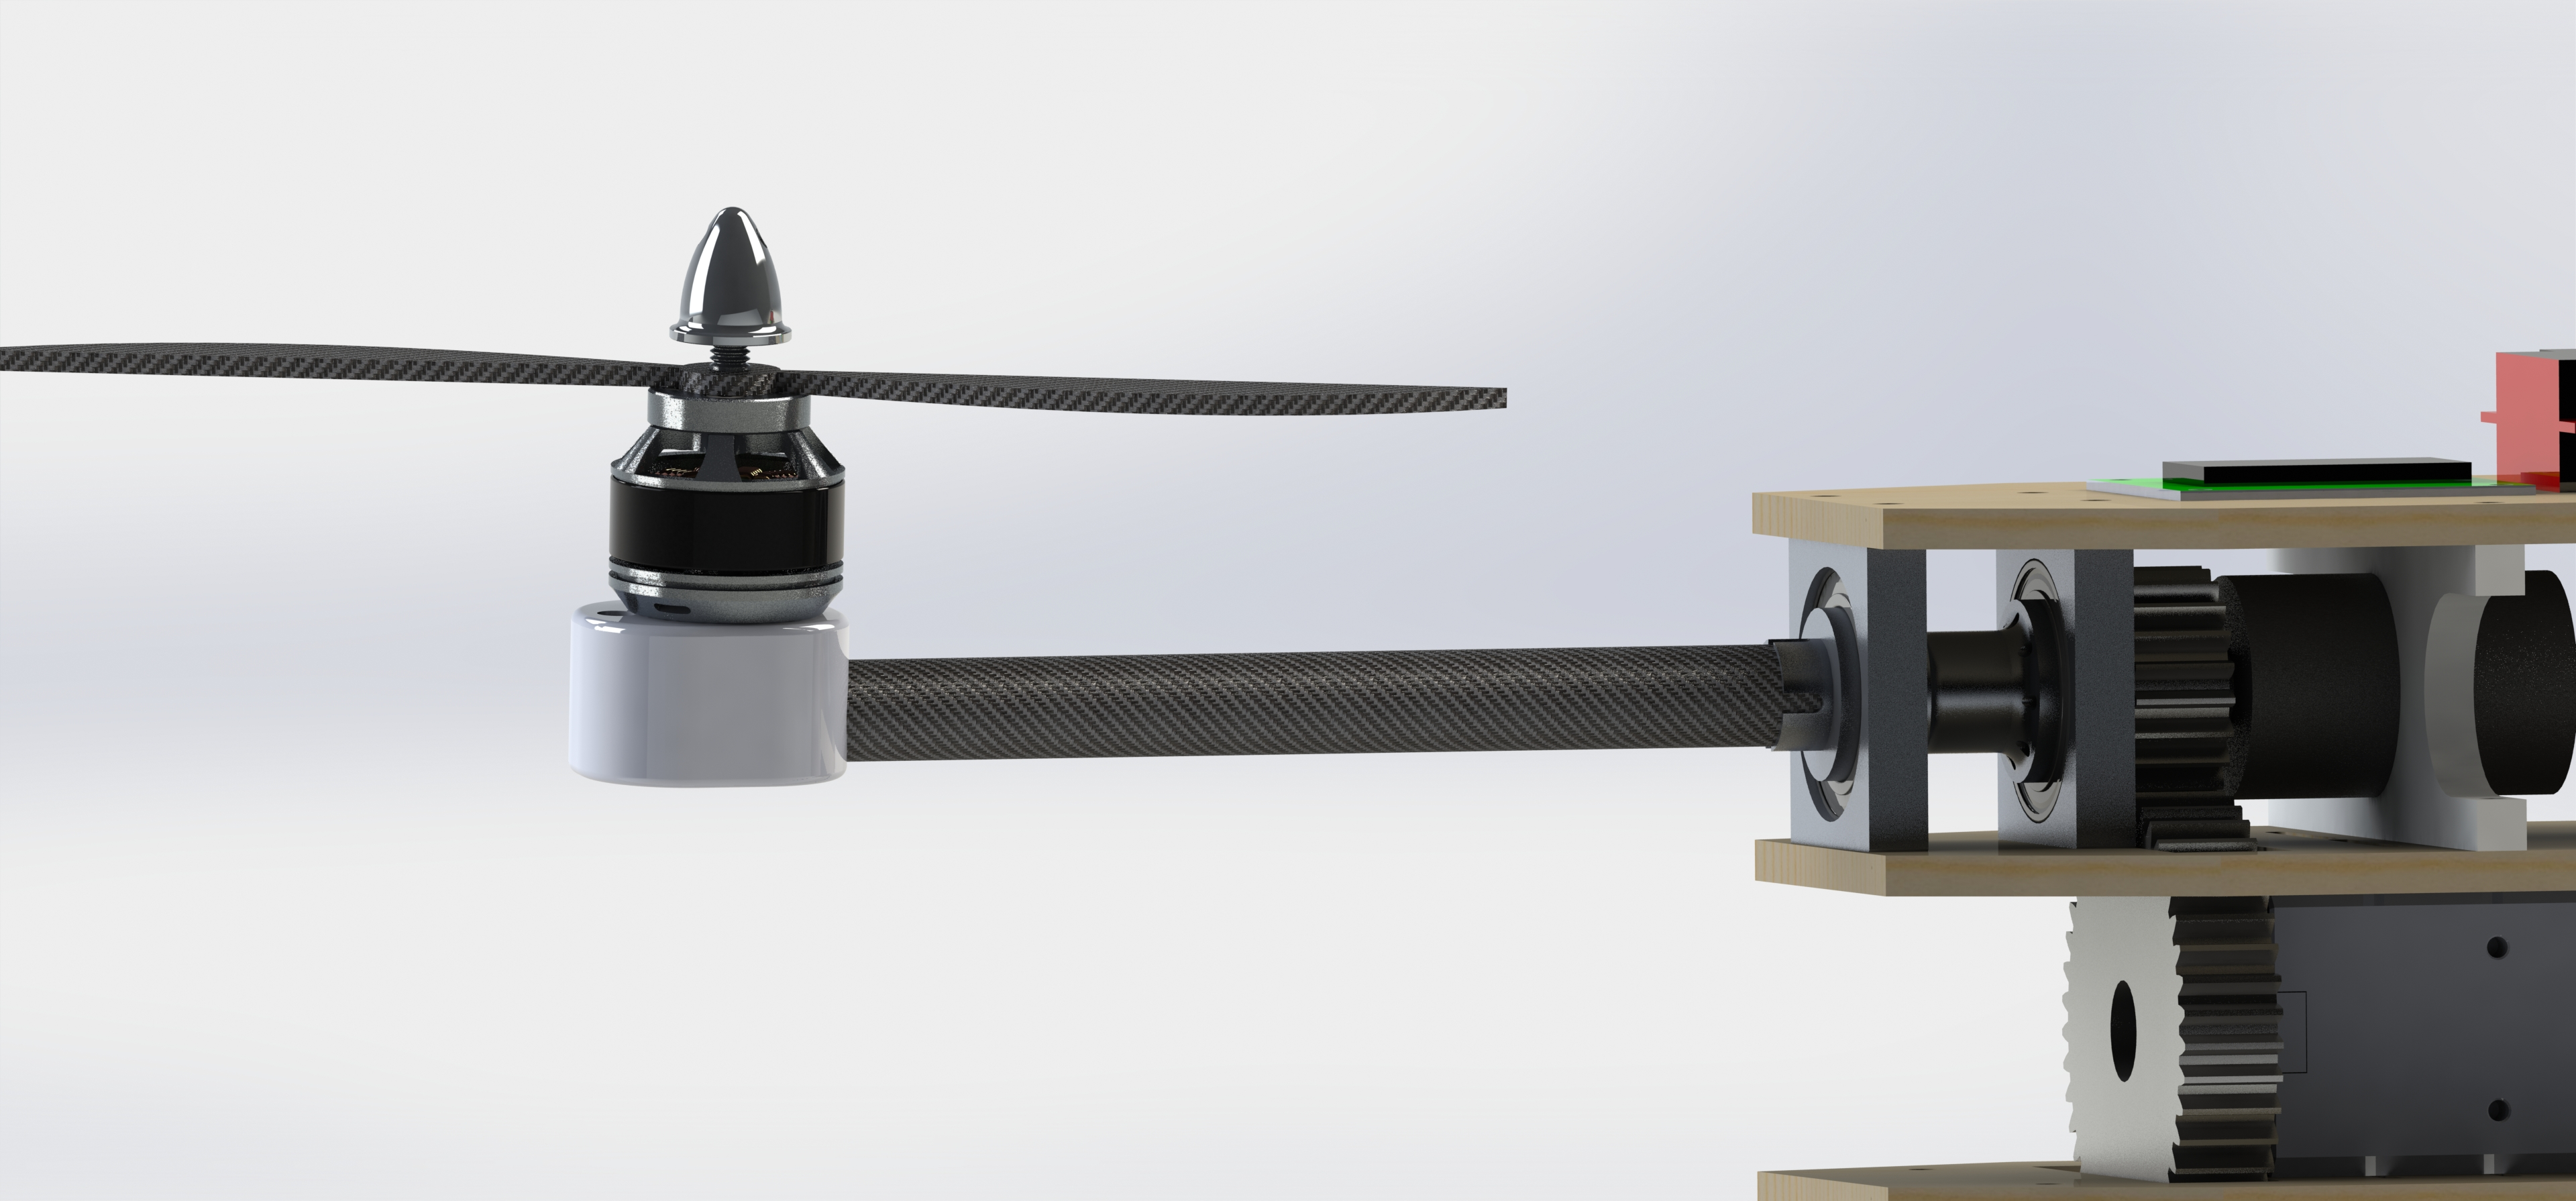
\includegraphics[scale=0.04]{pictures/zoom2}
\end{figure}
\end{frame}

\section{What are the next steps ?}
\begin{frame}{What are the next steps ?}
\begin{itemize}
\item To finish building it
\begin{figure}
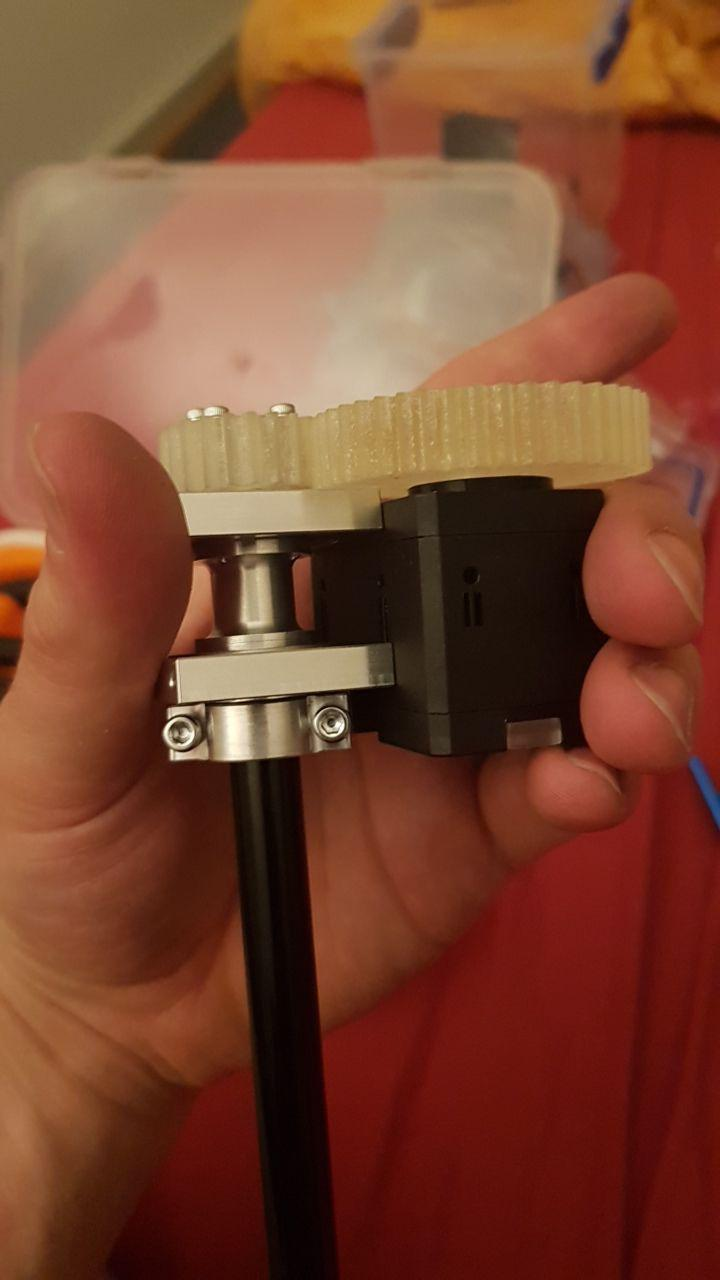
\includegraphics[scale=0.3]{pictures/build1}
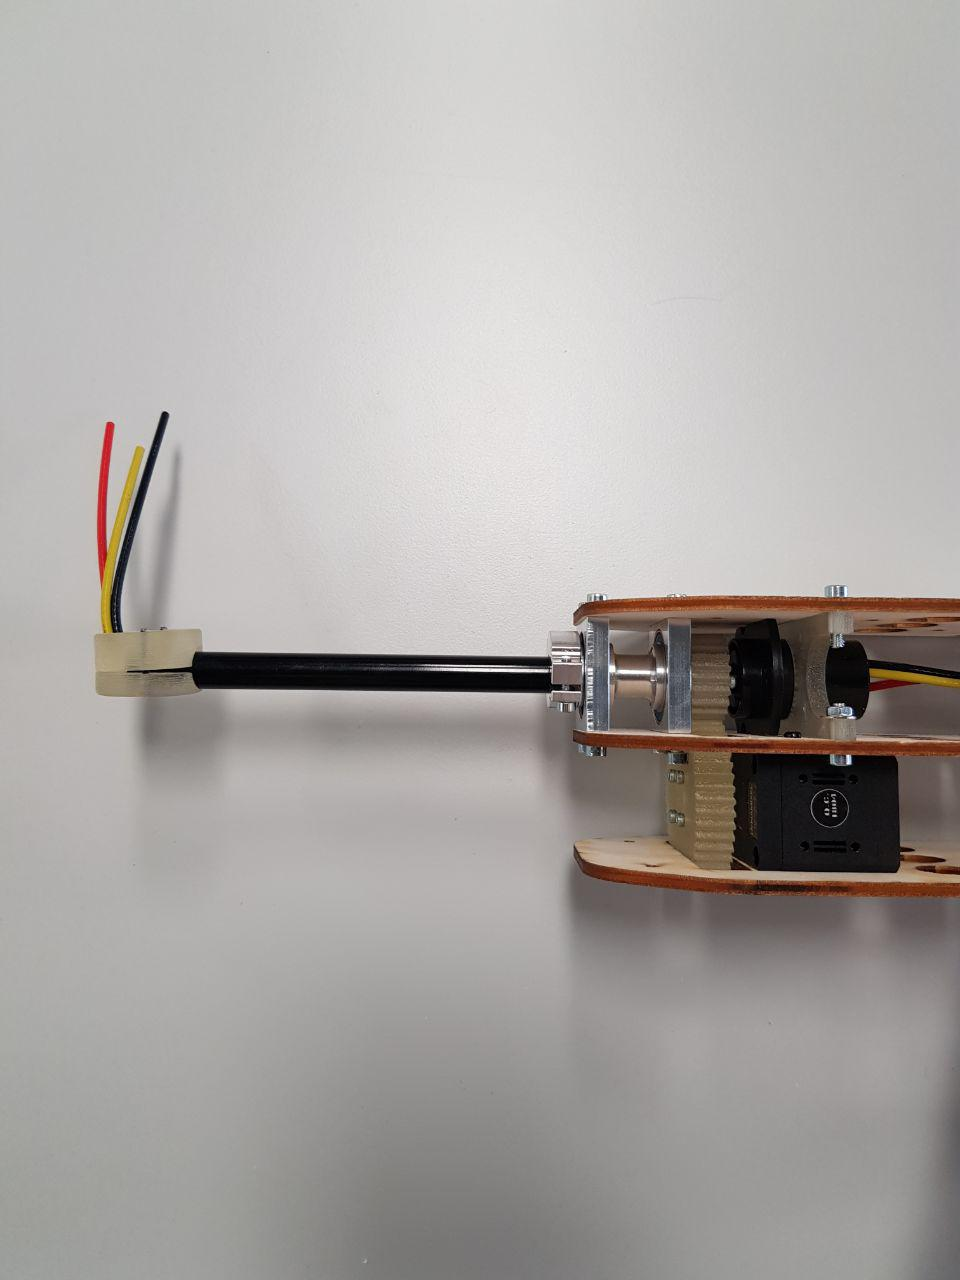
\includegraphics[scale=0.3]{pictures/build3}
\end{figure}
\end{itemize}
\end{frame}

\begin{frame}{What are the next step ?}
\begin{itemize}
\item Create the gazebo model
\begin{figure}
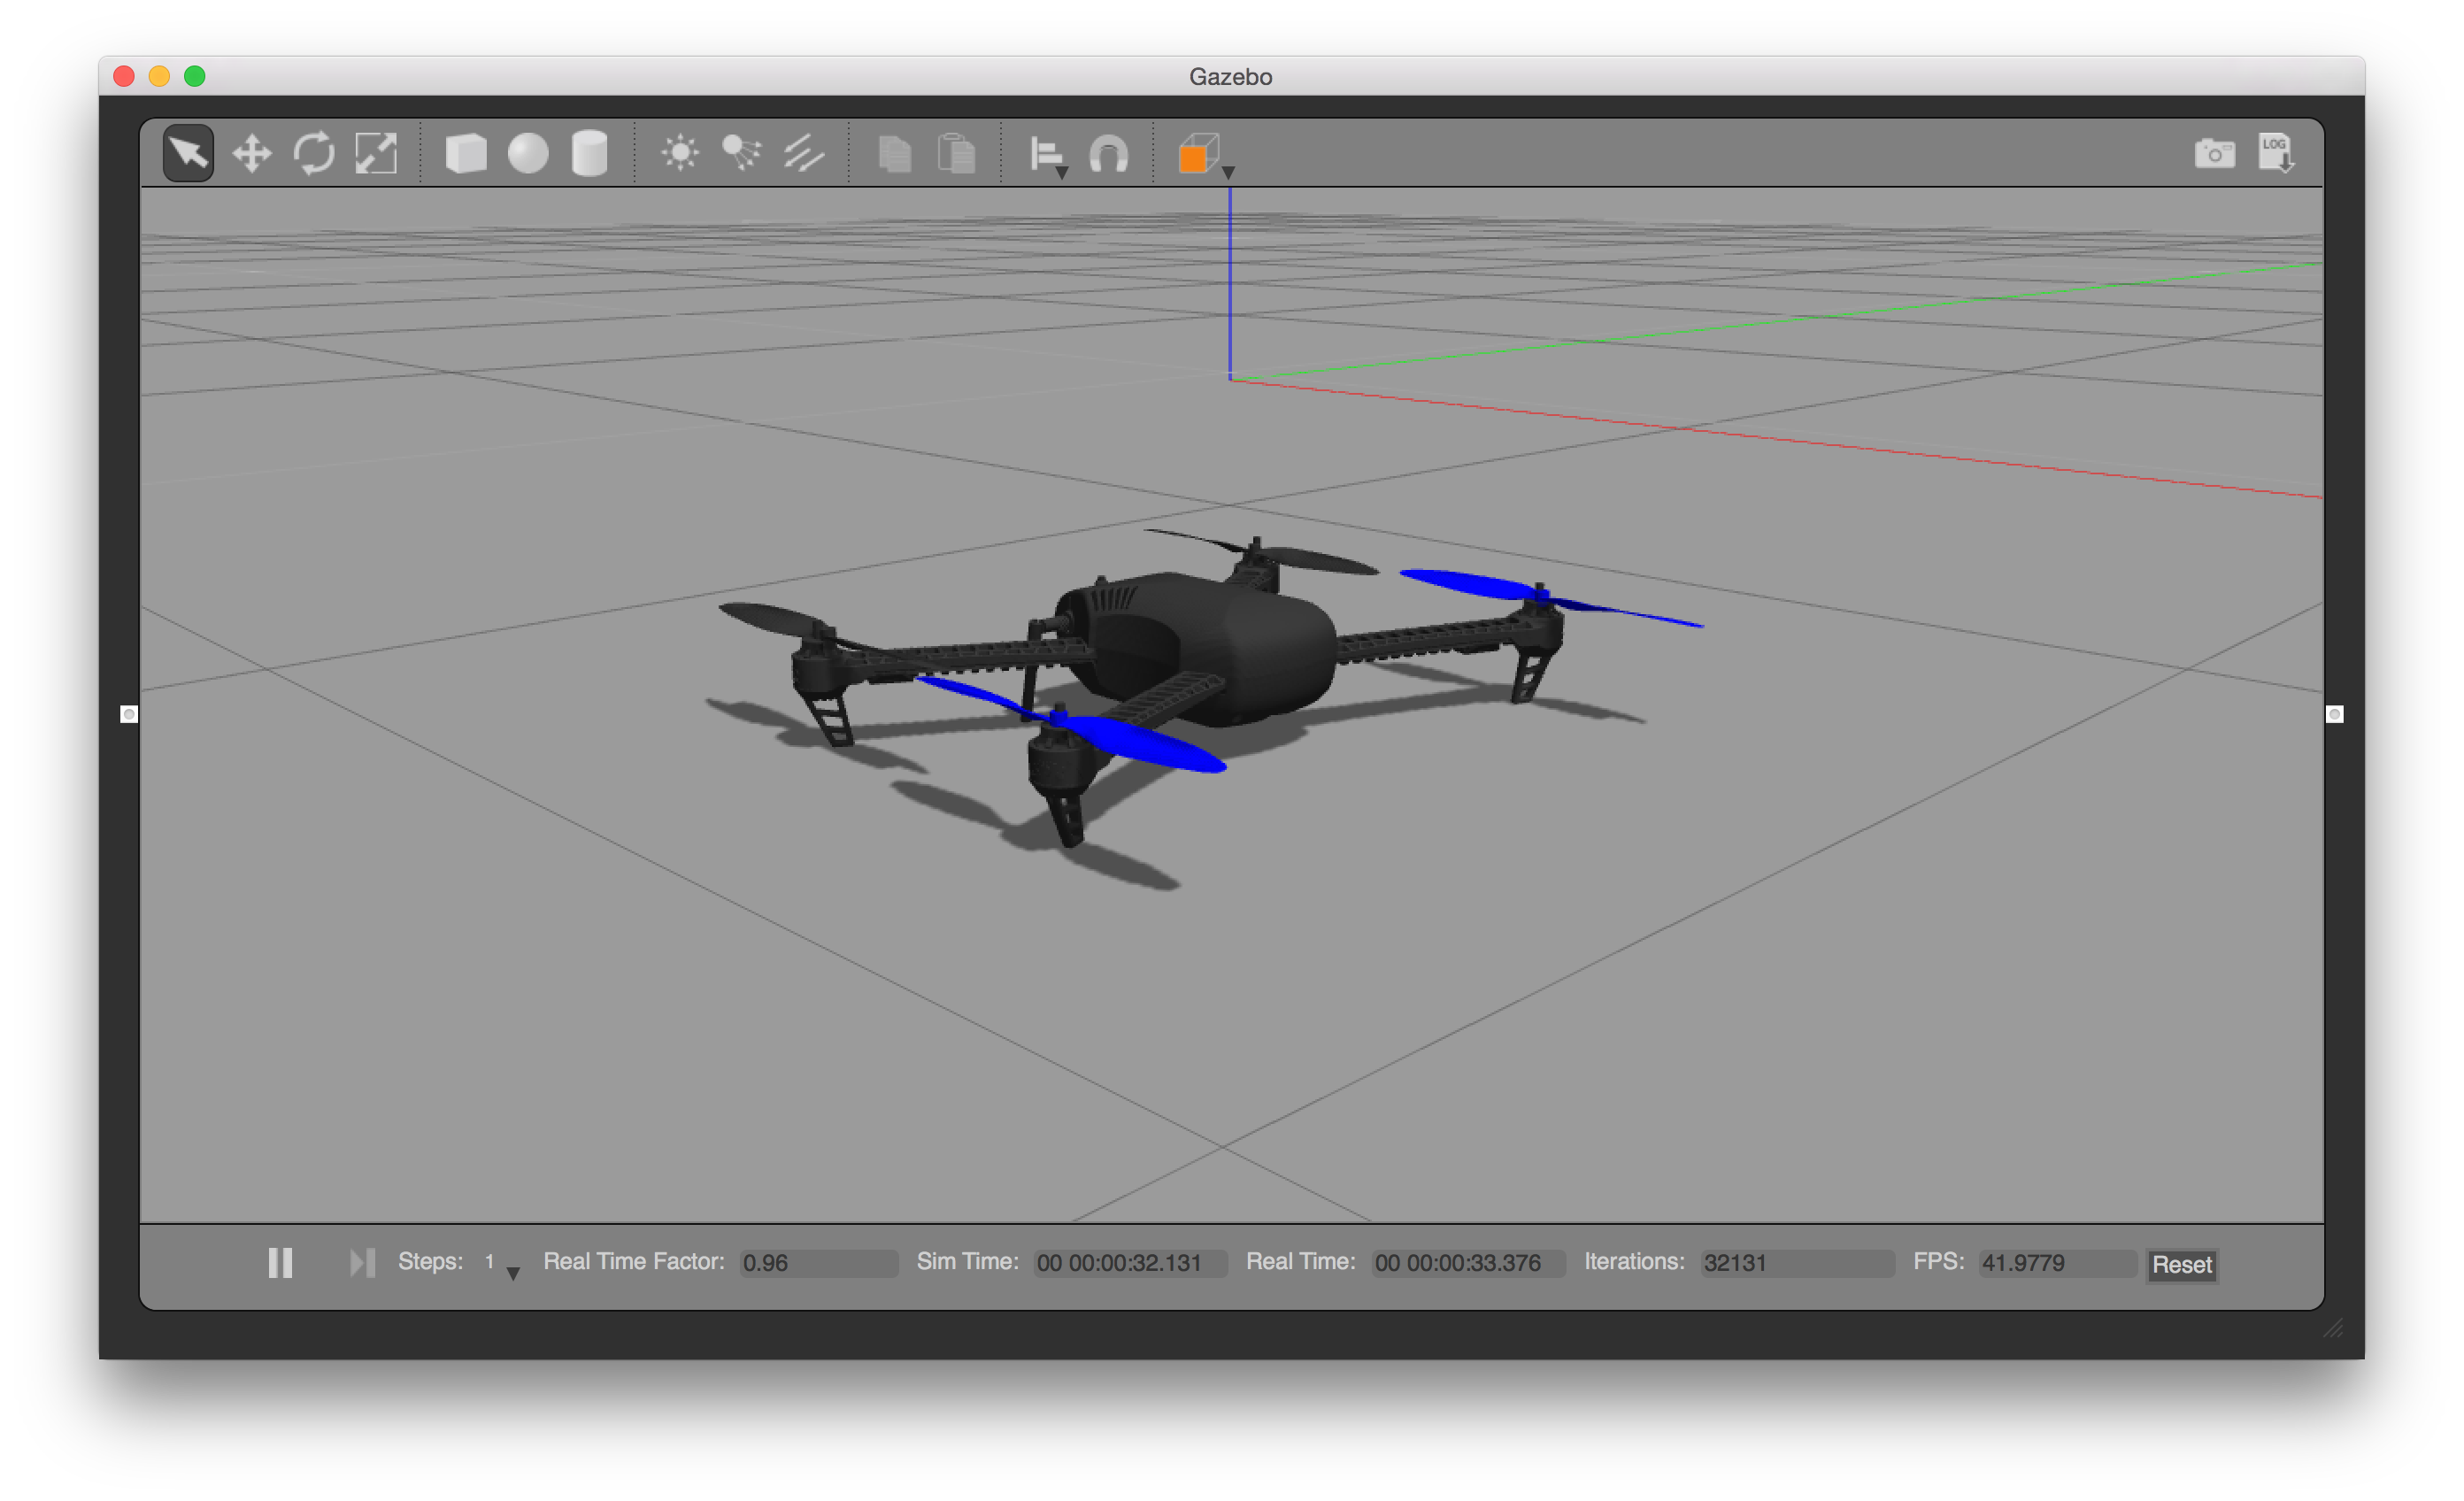
\includegraphics[scale=0.1]{pictures/gazebo}
\end{figure}
\item To develop the system for control
\item Bonus : test it in a real flight
\end{itemize}
\end{frame}

\section{References}
\begin{frame}{References}
\begin{itemize}
\item Picture - bicopter 1 : https://i.ytimg.com/vi/t36SHm18Gkc/maxresdefault.jpg
\item Picture - bicopter 2 : https://i.ytimg.com/vi/IDGvkzGSbVg/hqdefault.jpg
\item Picture - bicopter 3 : http://cdn3.volusion.com/ezdgu.nkdss/v/vspfiles/photos/ADX1501-7.jpg?1511770701
\end{itemize}
\end{frame}

\section{Questions}
\begin{frame}{}
\huge{Questions ?}
\end{frame}

\begin{frame}{}
\huge{Thank you for this project !}
\end{frame}



\end{document}

